% Options for packages loaded elsewhere
\PassOptionsToPackage{unicode}{hyperref}
\PassOptionsToPackage{hyphens}{url}
%
\documentclass[
]{book}
\usepackage{amsmath,amssymb}
\usepackage{iftex}
\ifPDFTeX
  \usepackage[T1]{fontenc}
  \usepackage[utf8]{inputenc}
  \usepackage{textcomp} % provide euro and other symbols
\else % if luatex or xetex
  \usepackage{unicode-math} % this also loads fontspec
  \defaultfontfeatures{Scale=MatchLowercase}
  \defaultfontfeatures[\rmfamily]{Ligatures=TeX,Scale=1}
\fi
\usepackage{lmodern}
\ifPDFTeX\else
  % xetex/luatex font selection
\fi
% Use upquote if available, for straight quotes in verbatim environments
\IfFileExists{upquote.sty}{\usepackage{upquote}}{}
\IfFileExists{microtype.sty}{% use microtype if available
  \usepackage[]{microtype}
  \UseMicrotypeSet[protrusion]{basicmath} % disable protrusion for tt fonts
}{}
\makeatletter
\@ifundefined{KOMAClassName}{% if non-KOMA class
  \IfFileExists{parskip.sty}{%
    \usepackage{parskip}
  }{% else
    \setlength{\parindent}{0pt}
    \setlength{\parskip}{6pt plus 2pt minus 1pt}}
}{% if KOMA class
  \KOMAoptions{parskip=half}}
\makeatother
\usepackage{xcolor}
\usepackage{longtable,booktabs,array}
\usepackage{calc} % for calculating minipage widths
% Correct order of tables after \paragraph or \subparagraph
\usepackage{etoolbox}
\makeatletter
\patchcmd\longtable{\par}{\if@noskipsec\mbox{}\fi\par}{}{}
\makeatother
% Allow footnotes in longtable head/foot
\IfFileExists{footnotehyper.sty}{\usepackage{footnotehyper}}{\usepackage{footnote}}
\makesavenoteenv{longtable}
\usepackage{graphicx}
\makeatletter
\def\maxwidth{\ifdim\Gin@nat@width>\linewidth\linewidth\else\Gin@nat@width\fi}
\def\maxheight{\ifdim\Gin@nat@height>\textheight\textheight\else\Gin@nat@height\fi}
\makeatother
% Scale images if necessary, so that they will not overflow the page
% margins by default, and it is still possible to overwrite the defaults
% using explicit options in \includegraphics[width, height, ...]{}
\setkeys{Gin}{width=\maxwidth,height=\maxheight,keepaspectratio}
% Set default figure placement to htbp
\makeatletter
\def\fps@figure{htbp}
\makeatother
\setlength{\emergencystretch}{3em} % prevent overfull lines
\providecommand{\tightlist}{%
  \setlength{\itemsep}{0pt}\setlength{\parskip}{0pt}}
\setcounter{secnumdepth}{5}
\usepackage{fontspec}
\usepackage{xltxtra}
\XeTeXlinebreaklocale "th_TH"
\XeTeXlinebreakskip = 0pt plus 1pt  
\usepackage{fonts-tlwg}

\setmainfont[Script=Thai,%
    Scale=MatchLowercase,%
    WordSpace=1.25,%
    Mapping=tex-text,]{TH Sarabun New}

%% ---- Load line spacing package ---- %%
\usepackage{setspace}

% Introducing hair space 
\newrobustcmd{\hrsp}{\ifmmode\mskip1mu\else\kern0.0625em\fi}





\usepackage{tcolorbox}

% Define a new tcolorbox environment
\newtcolorbox{hello}{
  colframe=red, % border color
  colback=red!10, % background color
  coltext=red, % text color
  boxrule=0.5mm, % border thickness
  left=1mm, % left margin
  right=1mm, % right margin
  top=1mm, % top margin
  bottom=1mm % bottom margin
}
\ifLuaTeX
  \usepackage{selnolig}  % disable illegal ligatures
\fi
\usepackage[]{natbib}
\bibliographystyle{apalike}
\usepackage{bookmark}
\IfFileExists{xurl.sty}{\usepackage{xurl}}{} % add URL line breaks if available
\urlstyle{same}
\hypersetup{
  pdftitle={SCMA104 Systems of Ordinary Differential Equations and Applications in Medical Science},
  pdfauthor={Pairote Satiracoo},
  hidelinks,
  pdfcreator={LaTeX via pandoc}}

\title{SCMA104 Systems of Ordinary Differential Equations and Applications in Medical Science}
\author{Pairote Satiracoo}
\date{2024-08-07}

\usepackage{amsthm}
\newtheorem{theorem}{Theorem}[chapter]
\newtheorem{lemma}{Lemma}[chapter]
\newtheorem{corollary}{Corollary}[chapter]
\newtheorem{proposition}{Proposition}[chapter]
\newtheorem{conjecture}{Conjecture}[chapter]
\theoremstyle{definition}
\newtheorem{definition}{Definition}[chapter]
\theoremstyle{definition}
\newtheorem{example}{ตัวอย่าง}[chapter]
\theoremstyle{definition}
\newtheorem{exercise}{Exercise}[chapter]
\theoremstyle{definition}
\newtheorem{hypothesis}{Hypothesis}[chapter]
\theoremstyle{remark}
\newtheorem*{remark}{Remark}
\newtheorem*{solution}{Solution}
\begin{document}
\maketitle

{
\setcounter{tocdepth}{1}
\tableofcontents
}
\chapter{หลักการและความสำคัญของแคลคูลัสและระบบสมการเชิงอนุพันธ์สามัญ}\label{uxe2buxe25uxe01uxe01uxe32uxe23uxe41uxe25uxe30uxe04uxe27uxe32uxe21uxe2auxe33uxe04uxe0duxe02uxe2duxe07uxe41uxe04uxe25uxe04uxe25uxe2auxe41uxe25uxe30uxe23uxe30uxe1auxe1auxe2auxe21uxe01uxe32uxe23uxe40uxe0auxe07uxe2duxe19uxe1euxe19uxe18uxe2auxe32uxe21uxe0d}

แคลคูลัสมีส่วนประกอบหลักที่สำคัญอยู่ 2 องค์ประกอบ คือ

\begin{enumerate}
\def\labelenumi{\arabic{enumi}.}
\item
  การหาอนุพันธ์ (differentiation) และ
\item
  การหาปริพันธ์ (Integration)
\end{enumerate}

การประยุกต์เรื่องการหาอนุพันธ์ในการแก้ปัญหาเบื้องต้นที่สำคัญในทางชีววิทยา หรือทางการแพทย์ ประกอบด้วย การหาอัตราการเปลี่ยนแปลงของปริมาณของตัวแปรที่เราสนใจ และการใช้แคลคูลัสในการแก้ปัญหาการหาค่าสูงสุดและค่าต่ำสุดของปัญหาหรือฟังก์ชันที่แสดงความสัมพันธ์ของตัวแปรที่เราสนใจ

ตัวอย่างการเปลี่ยนแปลงของปริมาณที่สนใจ เช่น ขนาดของประชากร จำนวนของผู้ติดเชื้อจากโรคทางเดินหายใจ ระดับนำ้ตาลในกระแสเลือด ปริมาณของยาที่มีอยู่ในกระแสเลือกหรือส่วนหนึ่งของร่างกาย โดยที่การเปลี่ยนแปลงดังกล่าวสามารถเปรียบเทียบได้กับเวลา ดังต่อไปนี้

\begin{itemize}
\item
  ประชากรในประเทศไทยปี พ.ศ. 2566 มีจำนวน 66.05 ล้านคน (ข้อมูลอ้างอิงจาก \href{https://www.boi.go.th/index.php?page=demographic}{สำนักงานคณะกรรมการส่งเสริมการลงทุน})
\item
  ข้อมูลจำนวนผู้รักษาตัวในโรงพยาบาลจากศูนย์ข้อมูล COVID-19 ระหว่างวันที่ 28 กรกฎาคม ถึงวันที่ 3 สิงหาคม พ.ศ. 2567 (ข้อมูลอ้างอิงจาก \href{https://www.facebook.com/informationcovid19?locale=th_TH}{ศูนย์ข้อมูล Covid-19})
\end{itemize}

\begin{figure}

\includegraphics[width=1\linewidth]{images/fig-covid-19} \caption{ข้อมูลจำนวนผู้รักษาตัวในโรงพยาบาลจากศูนย์ข้อมูล COVID-19}\label{fig:fig-covid-19}
\end{figure}

\begin{itemize}
\tightlist
\item
  การเปลี่ยนแปลงของระดับนำ้ตาลในเลือดระหว่างมืออาหารสามมือในหนึ่งวัน (รูปภาพอ้างอิงจาก \href{https://en.wikipedia.org/wiki/Blood_sugar_level}{Wikipedia: Blood Sugar Level})
\end{itemize}

\begin{figure}
\includegraphics[width=1\linewidth]{images/fig-blood-glucose} \caption{ความผันผวนของระดับน้ำตาลในเลือด (สีแดง) และฮอร์โมนอินซูลิน (สีน้ำเงิน) ในมนุษย์ระหว่างมื้ออาหารสามมื้อ}\label{fig:fig-blood-glucose}
\end{figure}

\begin{itemize}
\tightlist
\item
  การเปลี่ยนแปลงของปริมาณยาในกระแสเลือดที่เวลาต่างๆ สำหรับการให้ยาโดยวิธีต่างๆ (รูปภาพอ้างอิงจาก \href{https://www.mdpi.com/1420-3049/28/24/8038}{บทความทางวิชาการในฐานข้อมูล MDPI})
\end{itemize}

\begin{figure}
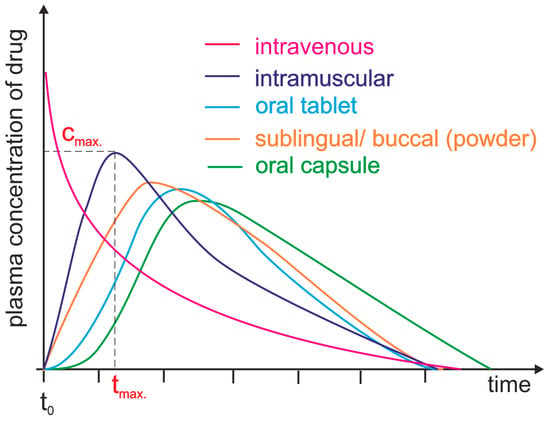
\includegraphics[width=1\linewidth]{images/fig-drug-absorption} \caption{ความเข็มข้นของยาในกระแสเลือดที่เวลาต่างๆ }\label{fig:fig-drug-absorption}
\end{figure}

ในการทำความเข้าใจการเปลี่ยนแปลงของปริมาณข้างต้นเทียบกับเวลา เราสามารถประยุกต์ใช้การสร้างแบบจำลองทางคณิตศาสตร์เพื่อมาใช้อธิบายการเปลี่ยนแปลงของปริมาณต่างๆ ที่เกี่ยวข้อง

\begin{quote}
\textbf{การสร้างแบบจำลองทางคณิตศาสตร์} เป็นกระบวนการอธิบายปัญหาหรือ ปรากฎการต่างๆ ที่เกิดขึ้นในธรรมชาติ โดยปกติแล้วจะอยู่ในรูปของสมการทางคณิตศาสตร์ ซึ่งแบบจำลองทางคณิตศาสตร์นี้จะช่วยให้อธิบายสิ่งต่างๆ ที่เกิดขึ้นในปัญหาหรือปรากฏที่สนใจ
\end{quote}

ตัวอย่างต่อไปนี้จะแสดงถึงแนวคิดในการประยุกต์ของแคลคูลัสที่เกี่ยวข้องกับอัตราการเปลี่ยนแปลงของ

\begin{example}
\protect\hypertarget{exm:exm1}{}\label{exm:exm1}ในการทดลองหนึ่ง นักวิจัยต้องการศึกษาการขยายพันธ์ของแบคทีเรียที่มีการการแบ่งตัวที่เรียกว่า binary fission (การแบ่งตัวแบบทวิภาค) ซึ่งแบคทีเรียจะมีการแบ่งจากหนึ่งเป็นสองเซลเท่าๆ กัน และได้ผลการทำลองดังต่อไปนี้
\end{example}

\begin{figure}
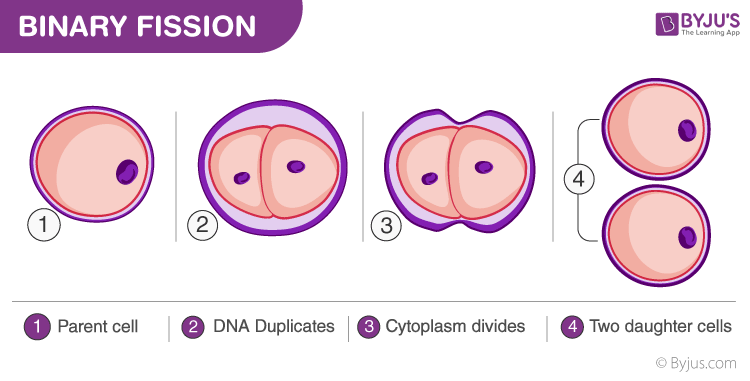
\includegraphics[width=1\linewidth]{images/fig-binary-fission} \caption{กระบวนการแบ่งตัวแบบทวิภาคของแบคทีเรีย}\label{fig:fig-binary-fission}
\end{figure}

(รูปอ้างอิงจาก \href{https://byjus.com/biology/binary-fission/}{BYJU's Learning Website} )

\begin{table}

\caption{\label{tab:bacteria-table}จำนวนของแบคทีเรียที่เวลา t ใดๆ}
\centering
\begin{tabular}[t]{l|r|r|r|r|r|r|r}
\hline
เวลา (10 นาที) & 0 & 1 & 2 & 3 & 4 & 5 & 6\\
\hline
จำนวนแบคทีเรีย & 1 & 2 & 4 & 8 & 16 & 32 & 64\\
\hline
\end{tabular}
\end{table}

ตาราง \ref{tab:bacteria-table} และรูปที่ \ref{fig:population-plot} แสดงการเปลี่ยนแปลงของจำนวนแบคทีเรียที่เวลาใดๆ ในตัวอย่างนี้การเปลี่ยนแปลงของจำนวนของแบคทีเรียที่เวลา \(t\) สามารถเขียนในรูปฟังก์ชัน \(N(t)\) ถ้าให้ \(N_0\) แทนจำนวนของแบคทีเรียตอนเริ่มการทดลอง แล้วแบบจำลองทางคณิตศาสตร์สำหรับการเพิ่มของจำนวนแบคทีเรียจะสามารถเขียนในรูปของสมการ

\begin{equation}
N(t) = N_0 \cdot 2 ^t, \quad t = 0,1,2, \ldots
\label{eq:population-growth}
\end{equation}

ในแบบจำลองทางคณิตศาสตร์นี้การเปลี่ยนแปลงของจำนวนแบคทีเรียที่เวลา \(t\) ใดๆ เพิ่มขึ้นในลักษณะที่เรียกว่า เอกซ์โพเนนเชียล (Exponential Population Growth)

\begin{figure}
\centering
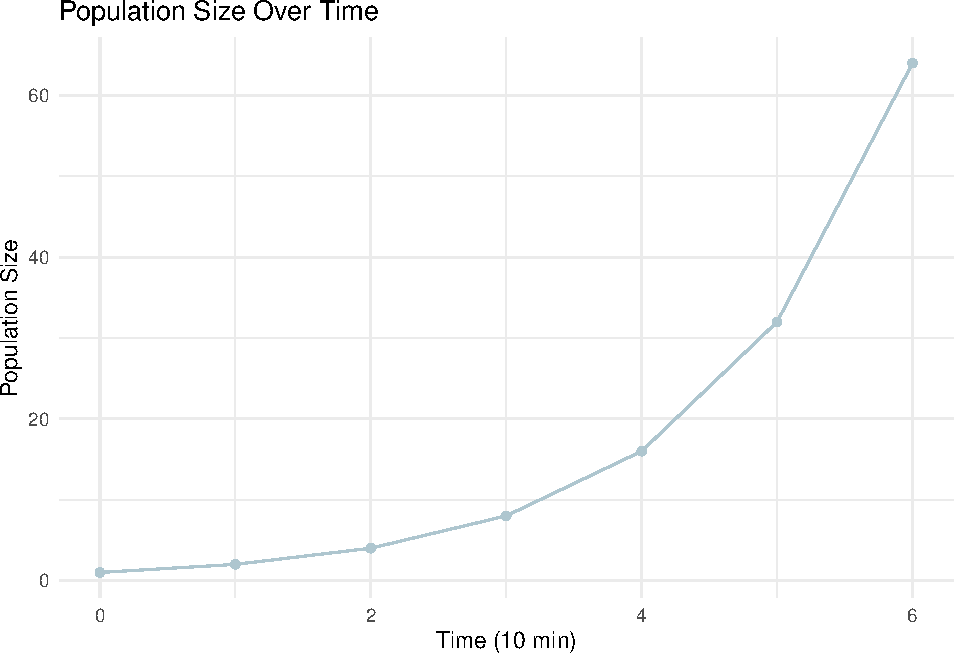
\includegraphics{SCMA104bookdownproj_files/figure-latex/population-plot-1.pdf}
\caption{\label{fig:population-plot}Population Size Over Time}
\end{figure}

\begin{example}
\protect\hypertarget{exm:exm2}{}\label{exm:exm2}ในการสร้างแบบจำลองทางคณิตศาสตร์ ในตัวอย่างของการขยายพันธ์แบคทีเรีย หรือในปัญหาอื่นๆ แทนที่เราจะพยายามหาความสัมพันธ์ หรือฟังก์ชัน \(N(t)\) ในรูปของเวลา \(t\) โดยตรง ถ้าเราทราบกระบวนการที่เกี่ยวข้องกับการอัตราการเปลี่ยนแปลงของตัวแปร \(N(t)\) นั้น เราสามารถนำมาใช้ในการสร้างแบบจำลองทางคณิตศาสตร์ ได้ดังต่อนี้ กระบวนการที่เกี่ยวข้องกับการเปลี่ยนแปลงของจำนวนแบคทีเรีย (การเพิ่มหรือลดลงของแบคทีเรีย) ที่เกิดขึ้นในระหว่างเวลา \(t\) และเวลา \(t + h\) เกิดจากจำนวนแบคทีเรียที่เพิ่มขึ้น (เกิดขึ้นมาใหม่) ในช่วงเวลาดังกล่าว และลดลงจากจำนวนแบคทีเรียที่ลดลง (ตายไป) ในช่วงเวลาดังกล่าวเช่นกัน ซึ่งเราสามารถเขียนในรูปของสมการได้ดังต่อไปนี้
\end{example}

\begin{align}
N(t + h) &= N(t) \\
&\quad + \text{จำนวนแบคทีเรียที่เกิดขึ้นใหม่ระหว่าง } t \text{ และ } t+h \\
&\quad - \text{จำนวนแบคทีเรียที่ตายไประหว่าง } t \text{ และ } t+h
\label{eq:population-growth-2}
\end{align}

ในที่นี้ ``\textbf{การเกิด}'' เราหมายถึงการเพิ่มจำนวนของแบคทีเรียจากหนึ่งเป็นสอง และเราจะกำหนดให้ \(h\) เป็นช่วงเวลาสั้นๆ (ซึ่งเราสามารถใช้ความรู้แคลคูลัสในการสร้างแบบจำลองทางคณิตศาสตร์ในรูปของสมการเชิงอนุพันธ์ (differential equation)) ในสมการ \eqref{eq:population-growth-2} ถ้าเราสมมติว่า การเพิ่มของแบคทีเรียเป็นสัดส่วนกับจำนวนแบคทีเรียที่มีอยู่ในขณะนั้น หรือเขียนในรูปของสมการได้ดังนี้

\[
\text{จำนวนแบคทีเรียที่เกิดใหม่ระหว่าง } t \text{ และ } t + h \approx b \cdot N \cdot h
\]

\[
\text{จำนวนแบคทีเรียที่ตายไประหว่าง } t \text{ และ } t + h \approx m \cdot N \cdot h
\]

โดยที่ค่าคงตัว \(b\) และ \(m\) ในสมการข้างต้น คือ อัตราการเกิด (birth rate) และอัตราการตาย (mortality rate)

เมื่อแทนจำนวนแบคทีเรียที่เกิดใหม่ และตายไประหว่างช่วงเวลาที่กำหนดลงในสมการ \eqref{eq:population-growth-2} จะได้สมการ

\begin{equation}
N(t + h) - N(t) = b\cdot N(t) \cdot h - m\cdot N(t) \cdot h
\label{eq:population-growth-3}
\end{equation}

เราสามารถจัดรูปสมการ \eqref{eq:population-growth-3} ได้ไหมในรูปของ\textbf{อัตราการเปลี่ยนแปลงเฉลี่ย}ของจำนวนแบคทีเรียในช่วงเวลาดังกล่าว ดังนี้

\begin{align}
\frac{N(t + h) - N(t)}{h} &= b\cdot N(t)  - m\cdot N(t)\\
\label{eq:population-growth-4}
\end{align}

ดังนั้น ถ้าเราให้ \(h\) เข้าใกล้ 0 ผ่านการหาค่าลิมิต เราจะได้อัตราการเปลี่ยนแปลงขณะหนึ่ง (instantaneous rate of change) และเขียนได้ในรูปของสมการเชิงอนุพันธ์ ดังนี้

\begin{align}
\frac{dN}{dt} = \lim_{h \rightarrow 0}\frac{N(t + h) - N(t)}{h} &= b\cdot N(t)  - m\cdot N(t)\\
\label{eq:population-growth-5}
\end{align}

ทั้งนี้ในการแก้สมการเชิงอนุพันธ์ \eqref{eq:population-growth-5} เพื่อให้ได้คำตอบที่แสดงจำนวนแบคทีเรีย \(N(t)\) ในรูปของฟังก์ชันของ \(t\) เราจะต้องกำหนดเงื่อนไขเพิ่มเติมที่เกี่ยวข้องกับจำนวนแบคทีเรีย \(N(t)\) ที่เวลา \(t\) หนึ่ง โดยทั่วไปเราจะกำหนดค่าเริ่มต้นของจำนวนแบคทีเรียที่ \(t = 0\) ดังนั้น ถ้าเรากำหนดเงื่อนไขเริ่มต้น (initial condition)

\begin{equation}
N(0) = N_0
\label{eq:population-growth-6}
\end{equation}

เราสามารถหาคำตอบของสมการเชิงอนุพันธ์ที่มีเงื่อนไขเริ่มต้นโดยวิธีการหาปริพันธ์ (Integration) ได้คำตอบของสมการดังนี้

\begin{equation}
N(t) = N_0 e^{(b-m)t}
\label{eq:population-growth-7}
\end{equation}

\begin{example}
\protect\hypertarget{exm:exm3}{}\label{exm:exm3}

ในการทดลองเลี้ยงยีสต์ในขวดทดลองที่มีอาหารเลี้ยงยีสต์ในปริมาณที่เหมาะสม ผู้ทำการทดลองสนใจที่จะประมาณค่าของยีสต์โดยอาศัยแบบจำลองการเปลี่ยนแปลงของประชากรที่อธิบายด้วยสมการ \eqref{eq:population-growth-7} กำหนดให้

\begin{itemize}
\item
  ภายใต้สภาวะของการทดลองที่เหมาะสม ยีสต์จะแบ่งตัวทุกๆ 90 นาที
\item
  ยีสต์มีครึ่งชีวิตเท่ากับ 1 สัปดาห์
\end{itemize}

จากข้อมูลดังกล่าว จงแสดงวิธีทำเพื่อหาคำตอบจากคำถามต่อไปนี้

\begin{enumerate}
\def\labelenumi{\arabic{enumi}.}
\item
  จงประมาณค่าของอัตราการเกิด \(b\) (1/ชั่วโมง) และอัตราการตาย \(m\) (1/ชั่วโมง)
\item
  เขียนแบบจำลองทางคณิตศาสตร์โดยใช้ค่า \(b\) และ \(m\) ที่ประมาณค่าได้ (สมการ \eqref{eq:population-growth-7})
\item
  ใช้เครื่องมือที่นักศึกษามีอยู่ในการวาดกราฟแสดงความสัมพันธ์ของจำนวนยีสต์ที่เวลาต่างๆ
\item
  เปรียบเทียบผลลัพธ์ที่ได้กับรูปภาพแสดงการเปลี่ยนแปลงของยีสต์จากการทดลองในห้องปฏิการ ตามรูปที่ \ref{fig:fig-yeast-cells} (รูปภาพอ้างอิงจาก \href{https://homework.study.com/explanation/a-graph-of-a-population-of-yeast-cells-in-a-new-laboratory-culture-as-a-function-of-time-is-shown-a-describe-how-the-rate-of-population-increase-varies-b-when-is-this-rate-highest-c-on-what-intervals-is-the-population-function-concave-upward-or-d.html}{https://homework.study.com/})
\end{enumerate}

\end{example}

\begin{figure}
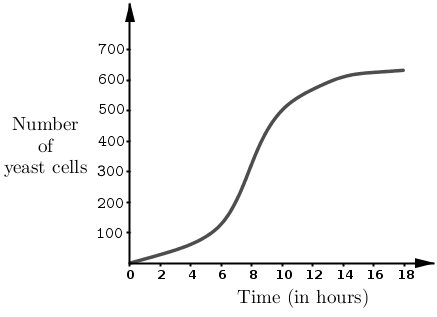
\includegraphics[width=0.5\linewidth]{images/fig-yeast-cells} \caption{กราฟการเจริญเติบโตของเซลล์ยีสต์}\label{fig:fig-yeast-cells}
\end{figure}

\begin{example}
\protect\hypertarget{exm:exm4}{}\label{exm:exm4}

จงใช้อินเทอร์เน็ตเพื่อค้นหาตัวอย่างแบบจำลองทางคณิตศาสตร์ที่อธิบายโดยสมการเชิงอนุพันธ์หรือระบบสมการเชิงอนุพันธ์ ข้อมูลที่ต้องการประกอบด้วย

\begin{enumerate}
\def\labelenumi{\arabic{enumi}.}
\item
  ค้นหาหน้าเว็บที่ให้ข้อมูลเกี่ยวกับแบบจำลองทางคณิตศาสตร์ในปัญหาที่นักศึกษาสนใจ
\item
  จดบันทึก URL ของหน้าเว็บ
\item
  เขียนสรุปสั้นๆ ว่าโมเดลนี้ใช้เพื่ออะไร
\end{enumerate}

\end{example}

โดยสรุป แคลคูลัสและสมการเชิงอนุพันธ์เป็นเครื่องมือสำคัญในการทำความเข้าใจว่าสิ่งต่างๆ เปลี่ยนแปลงไปอย่างไรและ แคลคูลัสช่วยให้เราวิเคราะห์อัตราการเปลี่ยนแปลงและพื้นที่ใต้เส้นโค้ง ในขณะที่สมการเชิงอนุพันธ์ช่วยให้เราสร้างแบบจำลองระบบที่ซับซ้อนในสาขาต่างๆ เช่น ฟิสิกส์ วิศวกรรม เศรษฐศาสตร์ และชีววิทยา แนวคิดทางคณิตศาสตร์เหล่านี้มีความสำคัญต่อการแก้ปัญหาในโลกแห่งความเป็นจริง เมื่อโลกของเราก้าวหน้ามากขึ้น ความสำคัญของแคลคูลัสและสมการเชิงอนุพันธ์ก็จะเพิ่มขึ้นอย่างต่อเนื่อง ซึ่งสนับสนุนความก้าวหน้าทางวิทยาศาสตร์และเทคโนโลยี

\chapter{The pool of tears}\label{the-pool-of-tears}

\begin{hello}

Custom block for latex

\end{hello}

\begin{tcolorbox}[colback=red!5!white,colframe=red!75!black,title=My nice heading] This is another \textbf{tcolorbox}.
\tcblower
Here, you see the lower part of the box.
\end{tcolorbox}

\begin{tcolorbox}
   This is a \textbf{tcolorbox}. This is a \textbf{tcolorbox}. This is a \textbf{tcolorbox}. This is a \textbf{tcolorbox}.    This is a \textbf{tcolorbox}. This is a \textbf{tcolorbox}. This is a \textbf{tcolorbox}. This is a \textbf{tcolorbox}.
\end{tcolorbox}

custom block for html

ทฤษฎีบท

An example of an admonition with a title.

\chapter{A caucus-race and a long tale}\label{a-caucus-race-and-a-long-tale}

\begin{tcolorbox}[colback=red!5!white,colframe=red!75!black,title=My nice heading] This is another \textbf{tcolorbox}.
\tcblower
Here, you see the lower part of the box.
\end{tcolorbox}

  \bibliography{book.bib}

\end{document}
